% !TeX root = ../report.tex

\section{Conclusions}
\subsection{Comparison of results}
Both analyses showed that:\\
- Problem in spatial allocation of important links such as "all the venues", as a matter of fact many users did not find the before mentioned link and failed or partially completed the task S6-T6\\
- The search bar influences the visibility of system status, the page appears to be frozen and many users were frustrated and were waiting for a long time\\

Differences:
- Some users found a number of problems that the inspectors missed during the inspection, we did not expect the search bar so much utilized\\
- Inspectors noticed immediately the main menu\\
- Users ignored the anchor links in pages like "university page" and "renting page"
% Comparison of the results achieved using the 2 methods
% - Problems priority and Suggestions for redesign
% - (Optional: Personal observations on the whole work performed: what did you learn?)
\subsection{Suggestions for redesign}

We have highlighted a few suggestions that may improve the user experience on the website:

\begin{itemize}
    \item In the desktop version of the website, the main header could take advantage of the larger width to show at least the main categories as landmarks that currently are shown only in the toggleable menu (\emph{Guide to the City}, \emph{Study}, \emph{Events}, ...), discarding the ``hamburger menu''. It could also show a dropdown when hovering on these categories that lists their content (e.g.: \emph{Study} > \emph{Welcome to Milano, Universities \& Academies, ...}), as show in Fig. \ref{fig:redesign-1}. The ``hamburger menu'' would still be present on tablet and smartphone versions of the website.
    \begin{figure}[!ht]
        \begin{minipage}{\linewidth}
            \centering
            \makebox[\textwidth][c]{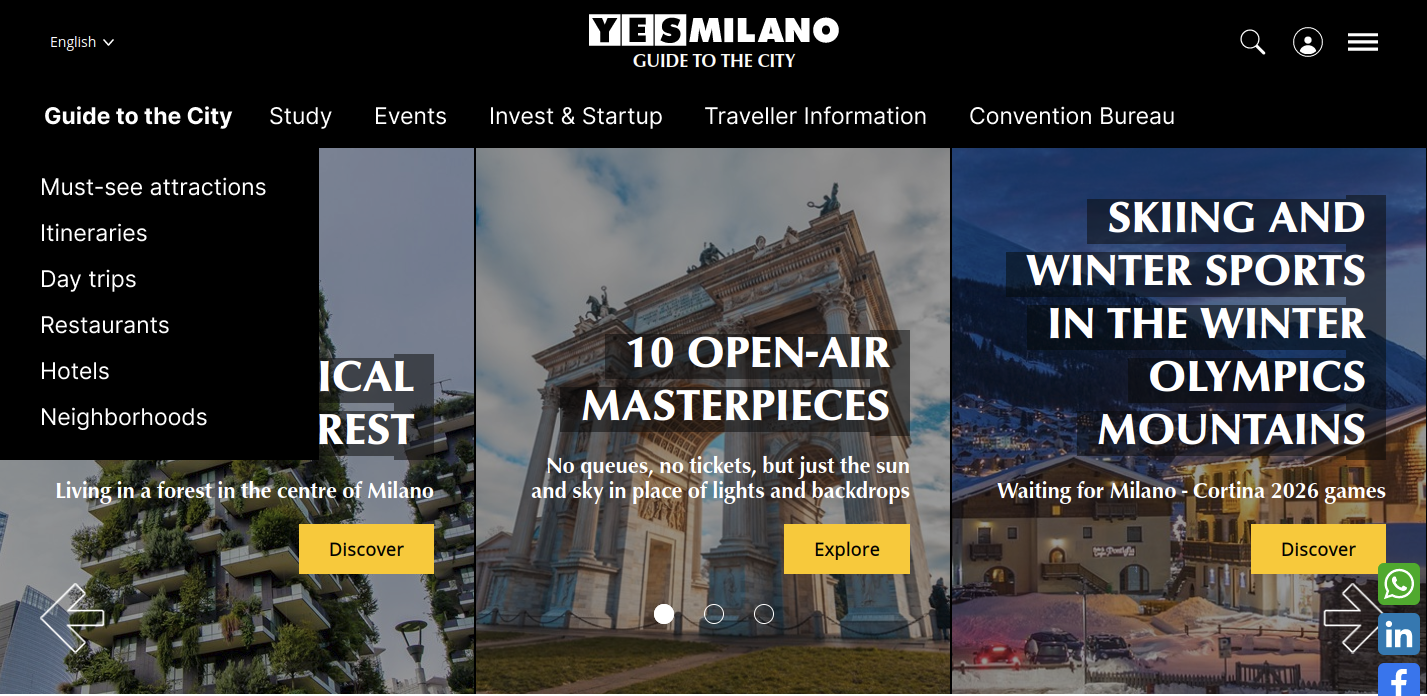
\includegraphics[width=0.8\textwidth]{images/redesign-1.png}}%
            \captionsetup{justification=centering}
            \caption{Redesign of the header including a list of main categories as landmarks with an opened dropdown for the \emph{Guide to the City} category.}
            \label{fig:redesign-1}
        \end{minipage}
    \end{figure}

    \item An important and missing menu item is the \emph{All the venues} link, which is only present in the footer. It's a useful page because it allows users to quickly filter through all the attractions and locations of the city. It should be moved in the menu and made reachable from the \emph{Guide to the City} page.
    
    \item The searchbar feature is often used by users, but its slowness is detrimental to the user experience. Search times and performance should be improved by optimizing the backend or resorting to third-party solutions (e.g.: Algolia, Elasticsearch, ...). It should be also made clear when the website is loading by showing a very visible spinner or a loading page, instead of waiting for the results to be ready and then redirecting the user to such page.
    
    \item Pages such as \emph{Itineraries}, \emph{Must-see attractions} or the various Event lists, which list many items, provide no way to filter their items. It would be useful to at least provide a filter by topic (i.e.: Art, Education, Fashion, ...)
    
    \item Anchor links at the top of pages such as \emph{Universities, Academies \& Schools in Milano} (Fig. \ref{fig:MC1-1}) or \emph{Rents} are daunting and hard to use: it would be better to reorganize them in a list (possibly grouped by category). These summaries could also be sticky and placed in a sidebar, so users can quickly navigate through the page sections.
    
    \item Breadcrumbs should always be present and be correct in most pages, since many pages have breadcrumbs that do not reflect the actions that the user took to reach that page, or the page relationship to other pages at all.
\end{itemize}
